\chapter{Actividad procesal}\label{cap:actividad-procesal}

Las pestañas de este capítulo registran lo que ocurre en el procedimiento
penal. Todas funcionan igual en cuanto a permisos:

\begin{itemize}
  \item \textbf{Administrador y Litigante asignado:} registran, corrigen y
        retiran.
  \item \textbf{Asistente legal asignado:} solo consulta y revisa el
        historial.
  \item \textbf{Expediente cerrado:} se puede consultar, pero no registrar
        cambios.
\end{itemize}

\nota{Qadra conserva lo que usted declara. Registrar una audiencia, una
resolución o un plazo no acredita por sí solo un acto judicial ni sus
efectos jurídicos.}

% ---------------------------------------------------------------------
\section{Cómo funcionan los registros}\label{sec:patron-registros}

Todos los formularios de este capítulo siguen el mismo recorrido:

\begin{enumerate}
  \item Llene el formulario.
  \item Haga clic en el botón de revisión (\textbf{Revisar registro},
        \textbf{Preparar registro}, \textbf{Preparar plazo}, según la
        pantalla).
  \item Revise el resumen y haga clic en el botón de confirmación
        (\textbf{Confirmar registro}, \textbf{Confirmar plazo}, etc.).
\end{enumerate}

\begin{table}[H]
  \centering
  \caption{Situaciones comunes en los formularios.}\label{tab:situaciones-comunes}
  \begin{tabularx}{\textwidth}{L{3.6cm} Y}
    \toprule
    \textbf{Situación} & \textbf{Qué hacer} \\
    \midrule
    Historial
      & Cada registro guarda sus cambios con autor y fecha. Use los botones
        \textbf{Ver historial de\ldots} de cada pestaña. \\
    Borrador guardado
      & Si cerró un formulario sin confirmar, aparece un botón
        \textbf{Retomar borrador de\ldots} para continuar. \\
    Otra persona cambió el registro
      & Haga clic en \textbf{Comparar con el registro actual}, revise las
        diferencias y elija \textbf{Usar esta base y conservar borrador}
        antes de confirmar. \\
    Resultado incierto
      & Si se pierde la respuesta, aparece \textbf{Resultado incierto}. Haga
        clic en \textbf{Consultar envío exacto} antes de intentar otra vez;
        consultar no repite el registro. \\
    Cerrar el formulario
      & \textbf{Cerrar formulario} descarta el borrador, pero no cancela un
        envío en curso. \\
    \bottomrule
  \end{tabularx}
\end{table}

% ---------------------------------------------------------------------
\section{Participantes}\label{sec:participantes}

\paraque Directorio de las personas e instituciones que intervienen en el
expediente. Registrar a una persona no le da acceso a Qadra.

\disponible Administrador y Litigante (registran); Asistente legal
(consulta).

\begin{table}[H]
  \centering
  \caption{Acciones en Participantes.}\label{tab:acciones-participantes}
  \begin{tabularx}{\textwidth}{L{4.4cm} Y}
    \toprule
    \textbf{Botón} & \textbf{Qué hace} \\
    \midrule
    \textbf{Agregar participante}     & Registra una identidad y su rol en el expediente. \\
    \textbf{Registrar ficha pendiente}& Registro manual rápido, para completarlo después. \\
    \textbf{Completar perfil}         & Convierte una ficha pendiente en un perfil completo. \\
    \textbf{Editar participante}      & Corrige los datos; la versión anterior queda en el historial. \\
    \textbf{Archivar participante} / \textbf{Reactivar participante}
                                      & Ordena el directorio; no cambia la situación jurídica. \\
    \textbf{Ver historial de cambios} & Muestra todas las versiones del registro. \\
    \bottomrule
  \end{tabularx}
\end{table}

\pasos\ Agregar un participante:
\begin{enumerate}
  \item En la pestaña \textbf{Participantes}, haga clic en
        \textbf{Agregar participante}.
  \item En \textbf{Datos de identidad}, elija el \textbf{Tipo de identidad}
        (\textbf{Persona} u \textbf{Órgano institucional}) y escriba el
        \textbf{Nombre de la persona}.
  \item En \textbf{Ficha de participación}, elija el
        \textbf{Tipo de participante} y llene los campos que aparezcan.
  \item Haga clic en \textbf{Revisar identidad y coincidencias}. Si Qadra
        encuentra personas parecidas, elija
        \textbf{Elegir identidad existente}, \textbf{Registrar otra identidad}
        o \textbf{Declarar persona distinta}.
  \item Haga clic en \textbf{Preparar registro} y después en
        \textbf{Confirmar registro}.
\end{enumerate}

\begin{figure}[H]
  \centering
  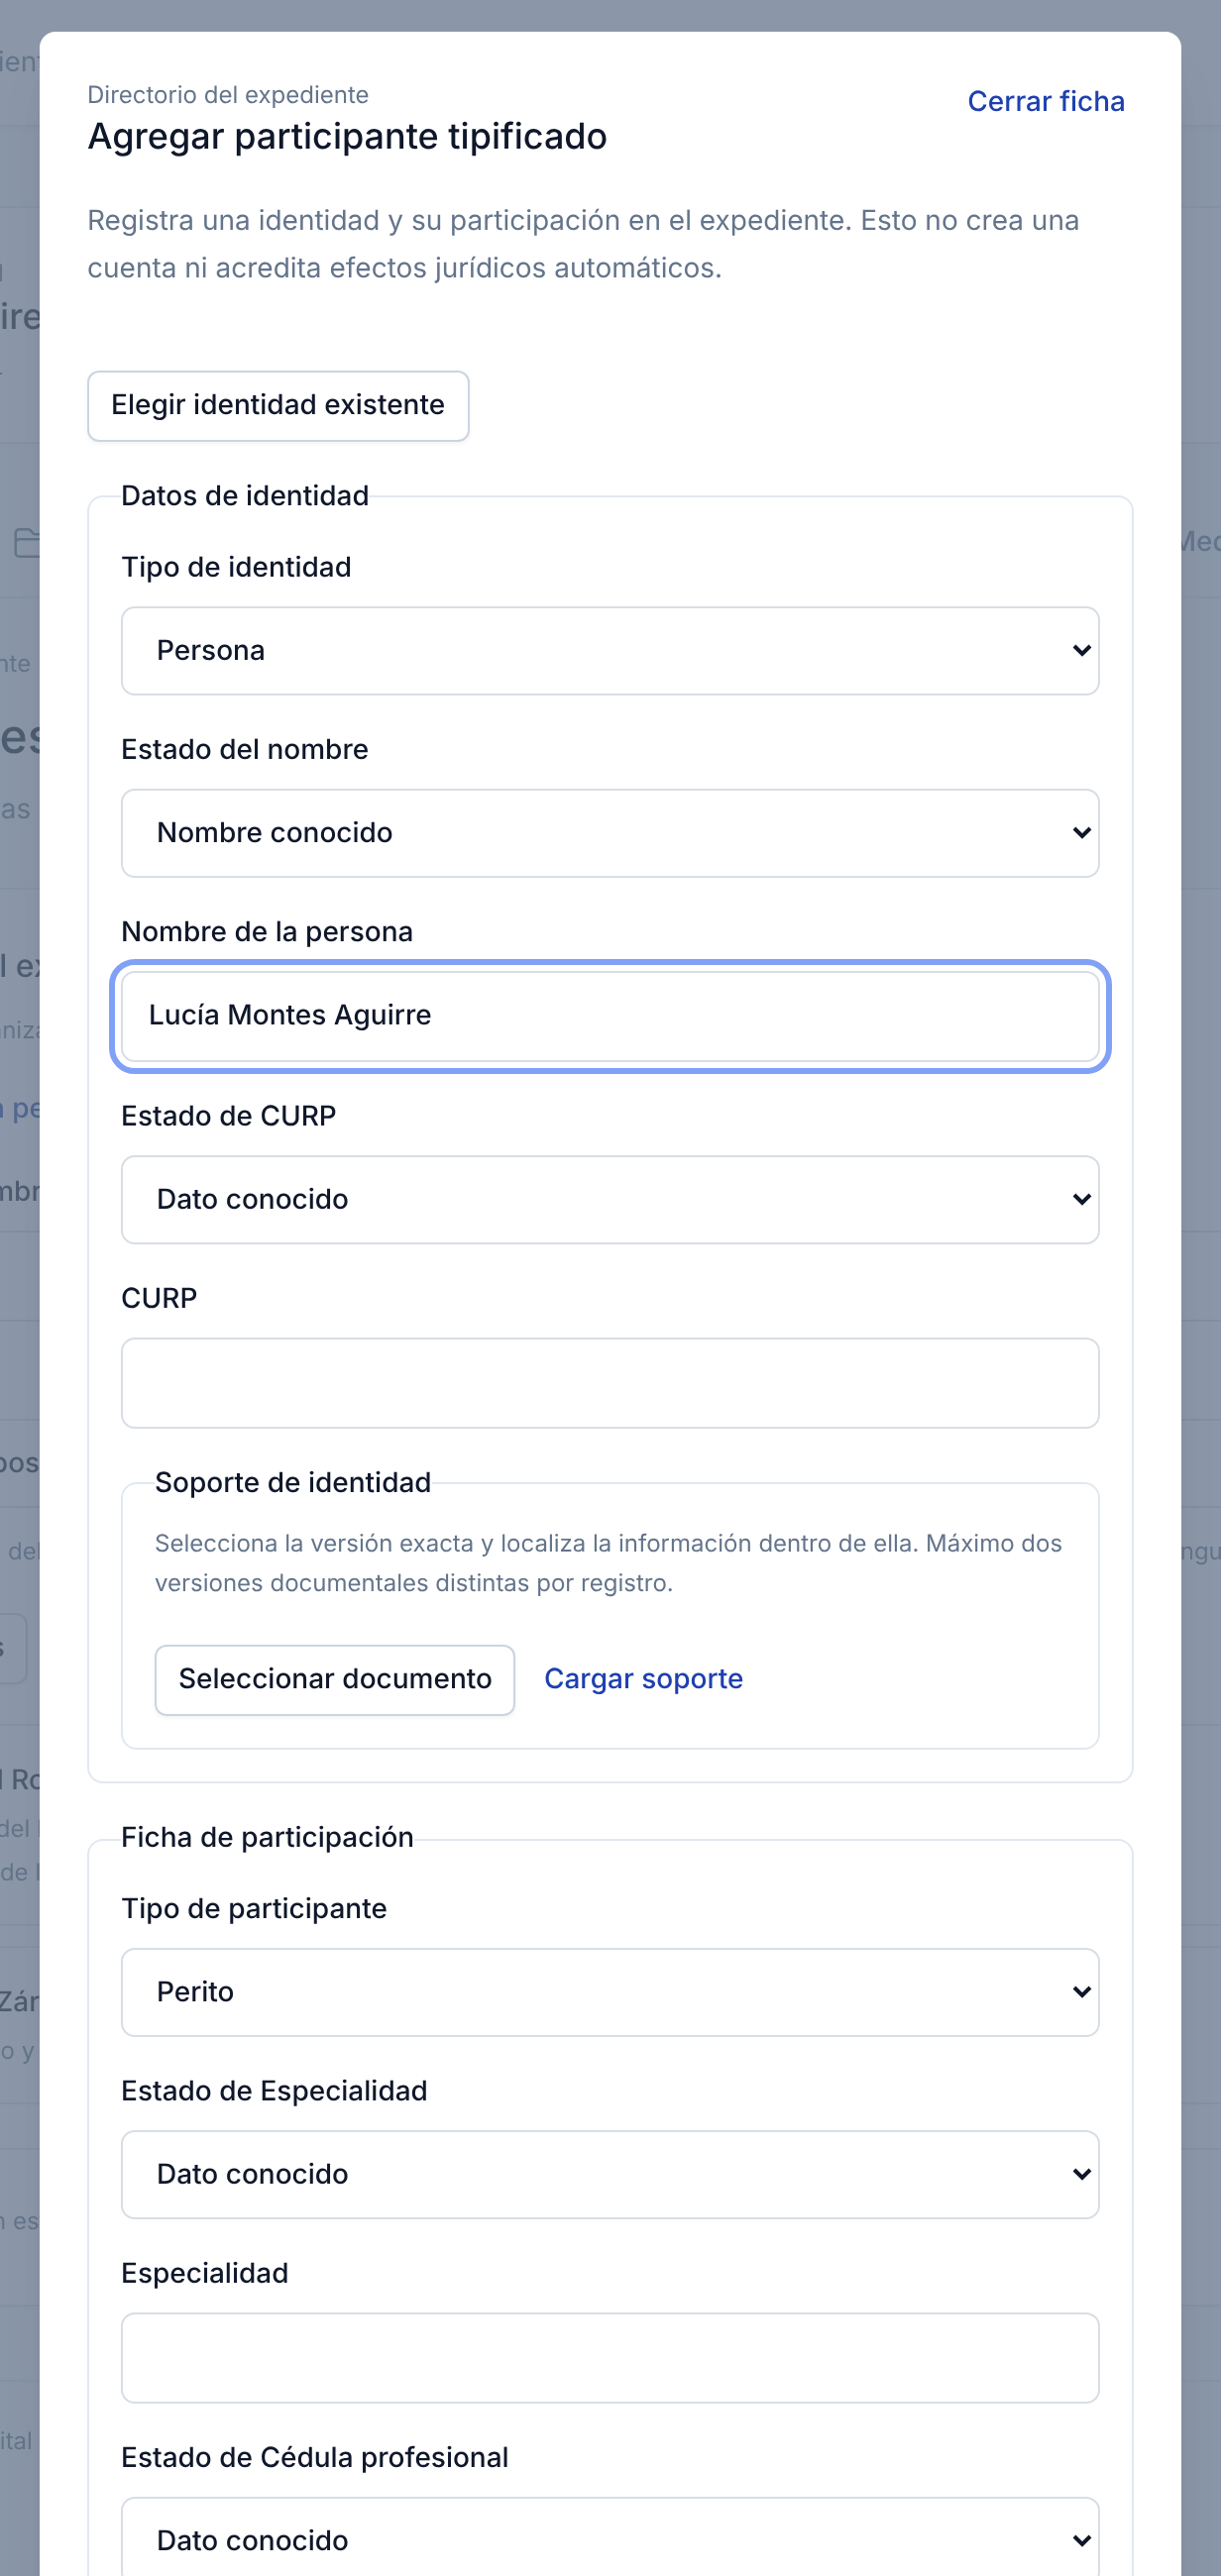
\includegraphics[width=0.9\textwidth,height=0.8\textheight,keepaspectratio]{capturas/A-27-agregar-participante.png}
  \caption{Registro de un participante.}
  \label{fig:manual-agregar-participante}
\end{figure}

\resultado El participante aparece en el \textbf{Directorio del expediente}.

\begin{itemize}
  \item Tipos disponibles: Imputado, Víctima u ofendido, Defensor,
        Ministerio Público, Asesor jurídico, Juez de control, Tribunal de
        enjuiciamiento, Perito, Policía, Supervisión de medidas cautelares y
        Otro.
  \item \textbf{Defensor} y \textbf{Juez de control} requieren certificado y
        firma: descargue la declaración con
        \textbf{Descargar declaración binaria}, fírmela con su herramienta y
        cargue el certificado y la firma con \textbf{Elegir certificado} y
        \textbf{Elegir firma}. Su clave privada nunca se sube a Qadra.
  \item Qadra nunca une a dos personas solo porque tengan el mismo nombre;
        usted decide en la revisión de coincidencias.
\end{itemize}

% ---------------------------------------------------------------------
\section{Etapas}\label{sec:etapas}

\paraque Registra la etapa procesal actual (Investigación, Intermedia o
Juicio) y sus cambios, con el documento que los respalda.

\disponible Administrador y Litigante (registran); Asistente legal
(consulta). Requiere la ficha penal completa.

\begin{table}[H]
  \centering
  \caption{Acciones en Etapas.}\label{tab:acciones-etapas}
  \begin{tabularx}{\textwidth}{L{4.6cm} Y}
    \toprule
    \textbf{Botón} & \textbf{Qué hace} \\
    \midrule
    \textbf{Registrar etapa actual}       & Declara la etapa en la que se encuentra un expediente sin etapa registrada. \\
    \textbf{Registrar paso a Intermedia}  & Registra el paso desde Investigación, con la acusación. \\
    \textbf{Registrar paso a Juicio}      & Registra el paso desde Intermedia, con el auto de apertura y su recepción. \\
    \textbf{Ver historial de etapas}      & Muestra todas las etapas registradas. \\
    \bottomrule
  \end{tabularx}
\end{table}

\pasos\ Registrar el paso a la siguiente etapa:
\begin{enumerate}
  \item En la pestaña \textbf{Etapas}, haga clic en
        \textbf{Registrar paso a Intermedia} (o
        \textbf{Registrar paso a Juicio}).
  \item Indique la fecha (por ejemplo, \textbf{Fecha de la acusación}). Si
        no conoce la hora, elija \textbf{Fecha sin hora conocida}.
  \item Elija el documento de soporte con \textbf{Elegir documento}, o
        súbalo con \textbf{Cargar soporte}. Debe ser PDF o DOCX.
  \item Haga clic en \textbf{Revisar registro} y después en
        \textbf{Registrar transición}.
\end{enumerate}

\begin{figure}[H]
  \centering
  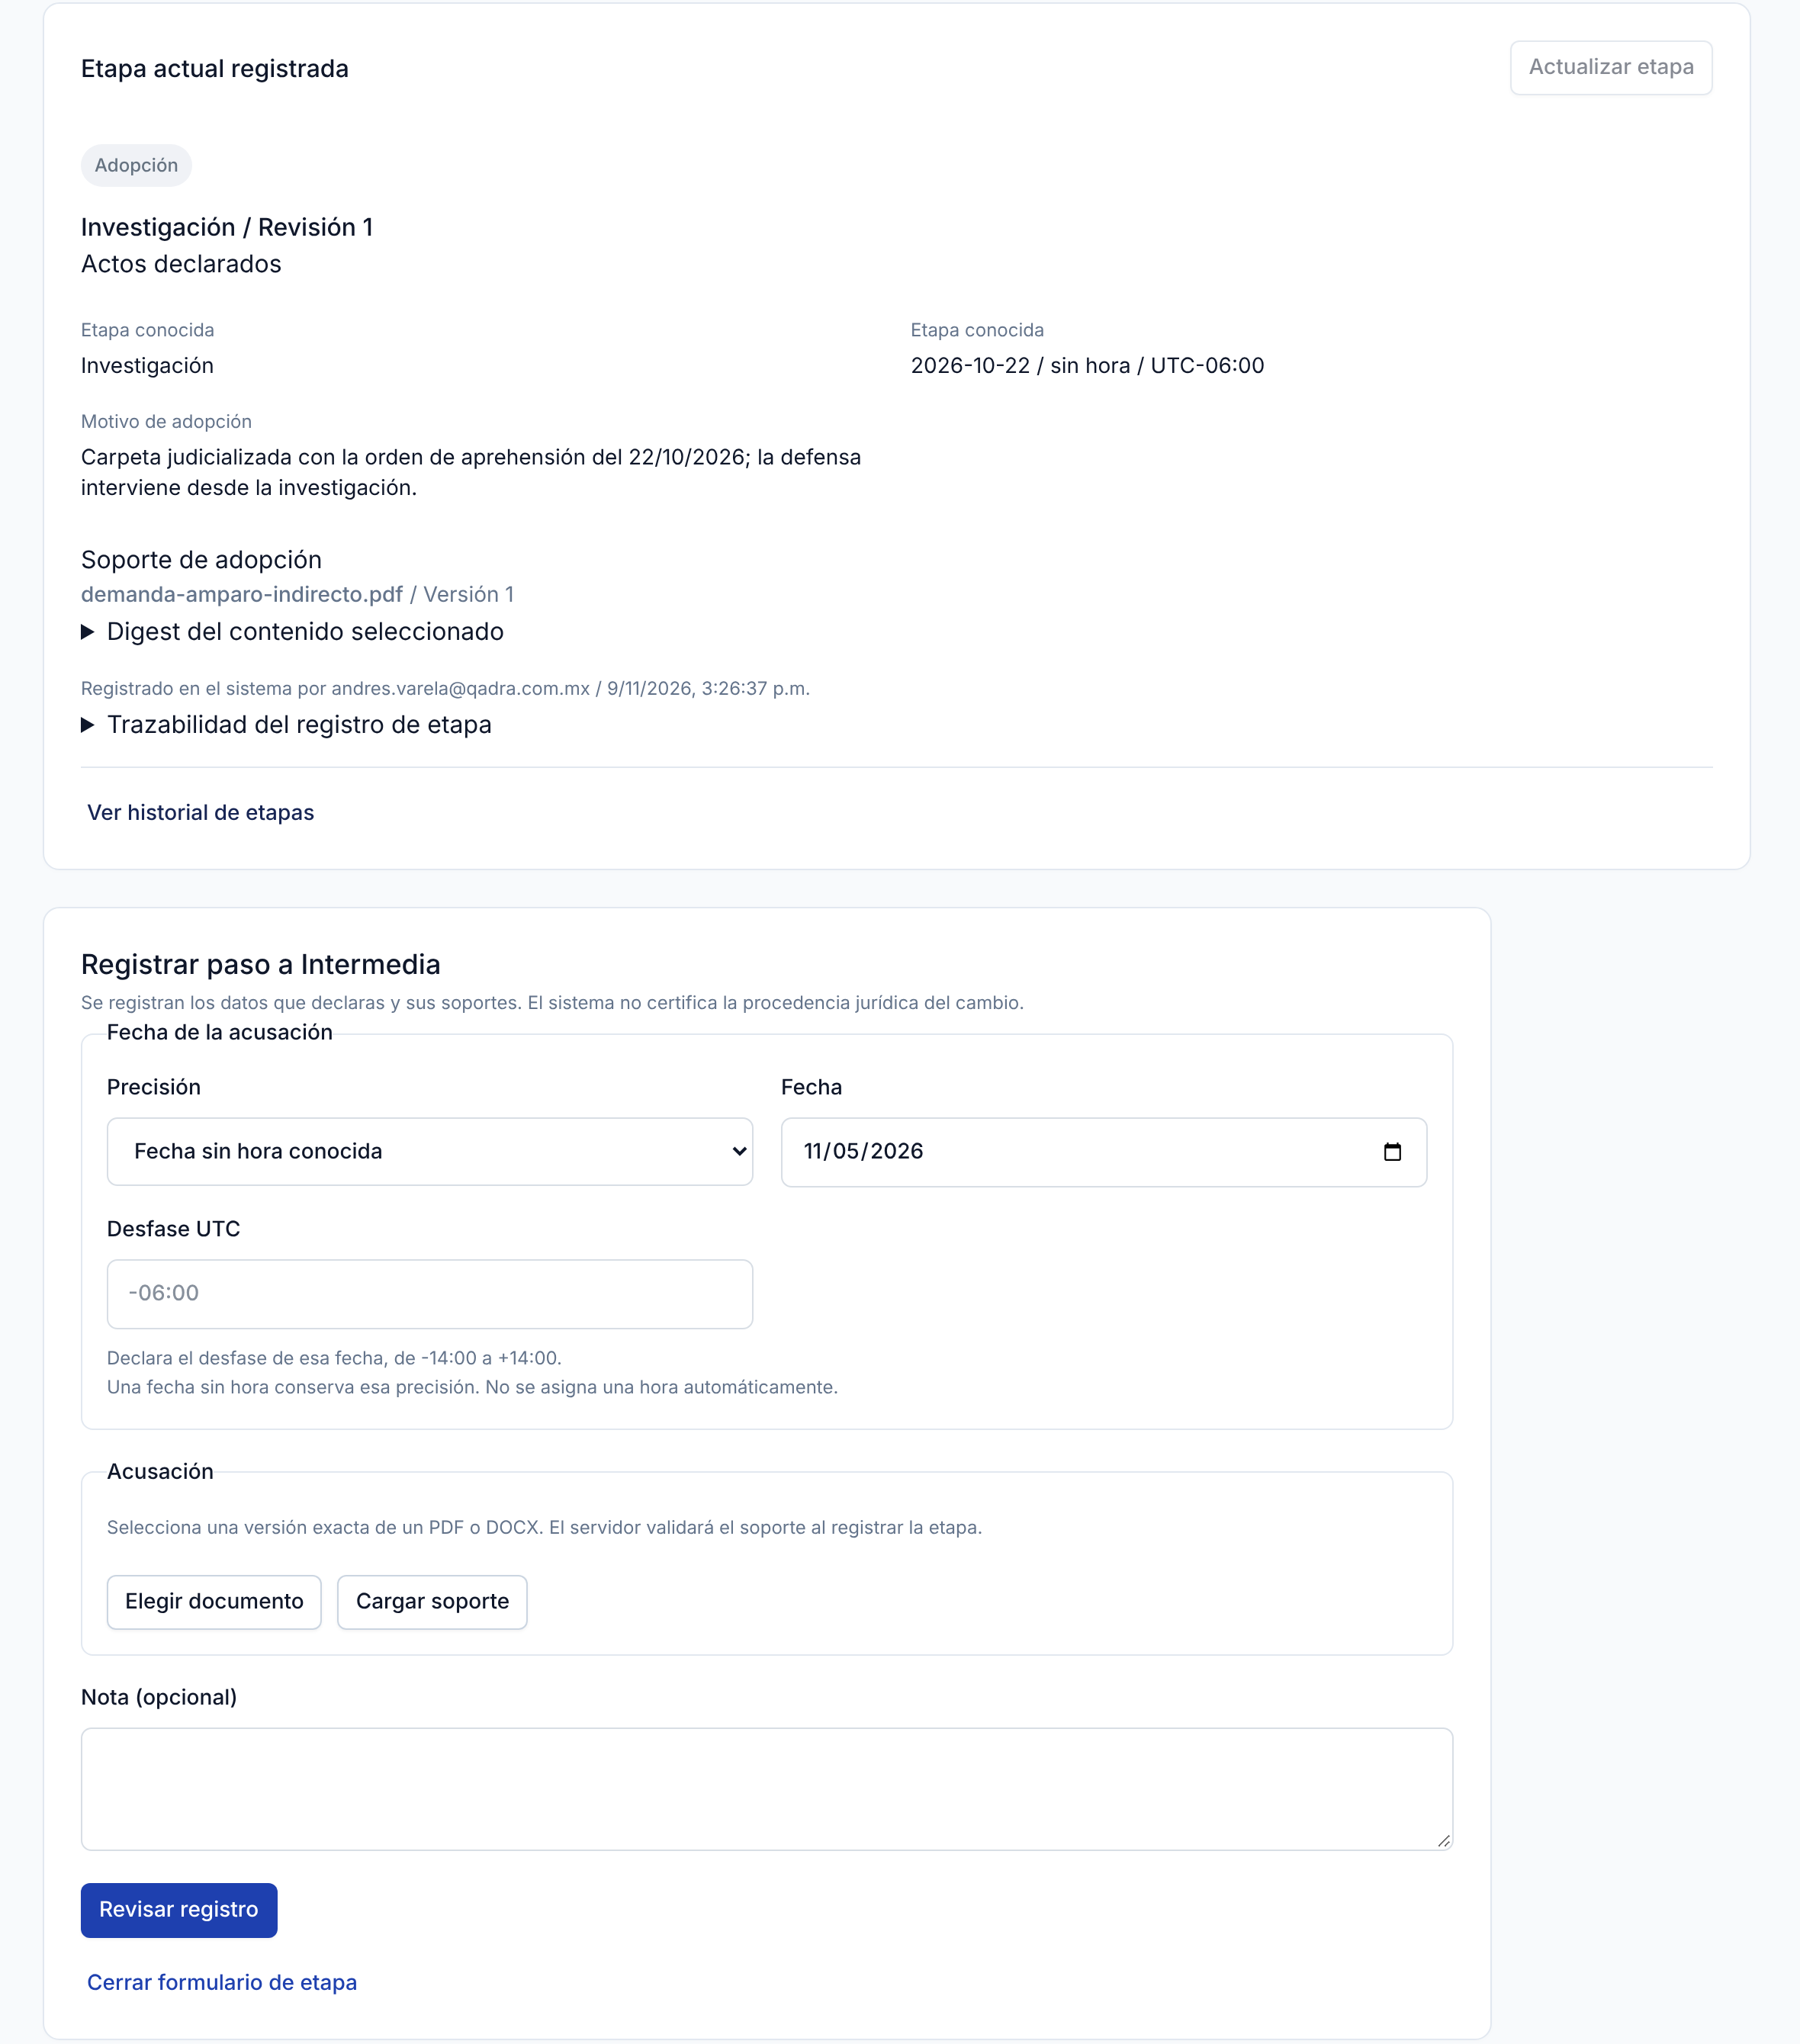
\includegraphics[width=0.9\textwidth,height=0.8\textheight,keepaspectratio]{capturas/A-28-etapas.png}
  \caption{Registro de un cambio de etapa.}
  \label{fig:manual-etapas}
\end{figure}

\resultado La pestaña muestra la nueva \textbf{Etapa actual registrada}.

\nota{Las etapas solo avanzan: Investigación, Intermedia y Juicio. Si la
ficha no está completa aparece \enquote{Completa la ficha penal para
registrar una etapa.} con el botón \textbf{Ir al resumen}.}

% ---------------------------------------------------------------------
\section{Audiencias}\label{sec:audiencias}

\paraque Programa audiencias, registra lo que ocurrió en ellas y conserva
cada cambio. También reúne las audiencias cautelares.

\disponible Administrador y Litigante (registran); Asistente legal
(consulta). Requiere la ficha penal completa y una etapa registrada.

\begin{table}[H]
  \centering
  \caption{Acciones en Audiencias.}\label{tab:acciones-audiencias}
  \begin{tabularx}{\textwidth}{L{4.6cm} Y}
    \toprule
    \textbf{Botón} & \textbf{Qué hace} \\
    \midrule
    \textbf{Programar audiencia}         & Registra una audiencia nueva. \\
    \textbf{Corregir o reprogramar}      & Cambia fecha, sede u otros datos, con su motivo. \\
    \textbf{Cancelar audiencia}          & Cancela la audiencia, con su motivo. \\
    \textbf{Ver sesiones y resultados}   & Registra qué ocurrió: \textbf{Registrar sesión o acto}, \textbf{Registrar continuación}, \textbf{Rectificar registro} o \textbf{Retirar registro}. \\
    \textbf{Registrar resultado y plazo} & Guarda el resultado y el plazo que genera en un solo paso. \\
    \textbf{Programar audiencia cautelar}& Convoca una audiencia de imposición o revisión de medidas cautelares. \\
    \textbf{Ver historial de audiencias} & Muestra todas las versiones de la audiencia. \\
    \bottomrule
  \end{tabularx}
\end{table}

\pasos\ Programar una audiencia:
\begin{enumerate}
  \item En la pestaña \textbf{Audiencias}, haga clic en
        \textbf{Programar audiencia}.
  \item Elija el \textbf{Tipo de audiencia}: Inicial, Intermedia, Debate de
        juicio o Individualización de sanciones y reparación del daño. Debe
        corresponder a la etapa registrada.
  \item Elija la \textbf{Modalidad} (\textbf{Presencial} o
        \textbf{Videoconferencia}), la fecha, la hora y la
        \textbf{Sede o conexión}.
  \item Agregue los participantes previstos: haga clic en
        \textbf{Elegir participante}, abra la ficha con
        \textbf{Consultar ficha: }\emph{nombre} y confirme con
        \textbf{Vincular esta revisión}. Repita para cada persona; la lista
        aparece en \textbf{Participantes previstos}.
  \item Haga clic en \textbf{Revisar registro} y después en
        \textbf{Confirmar registro}.
\end{enumerate}

\begin{figure}[H]
  \centering
  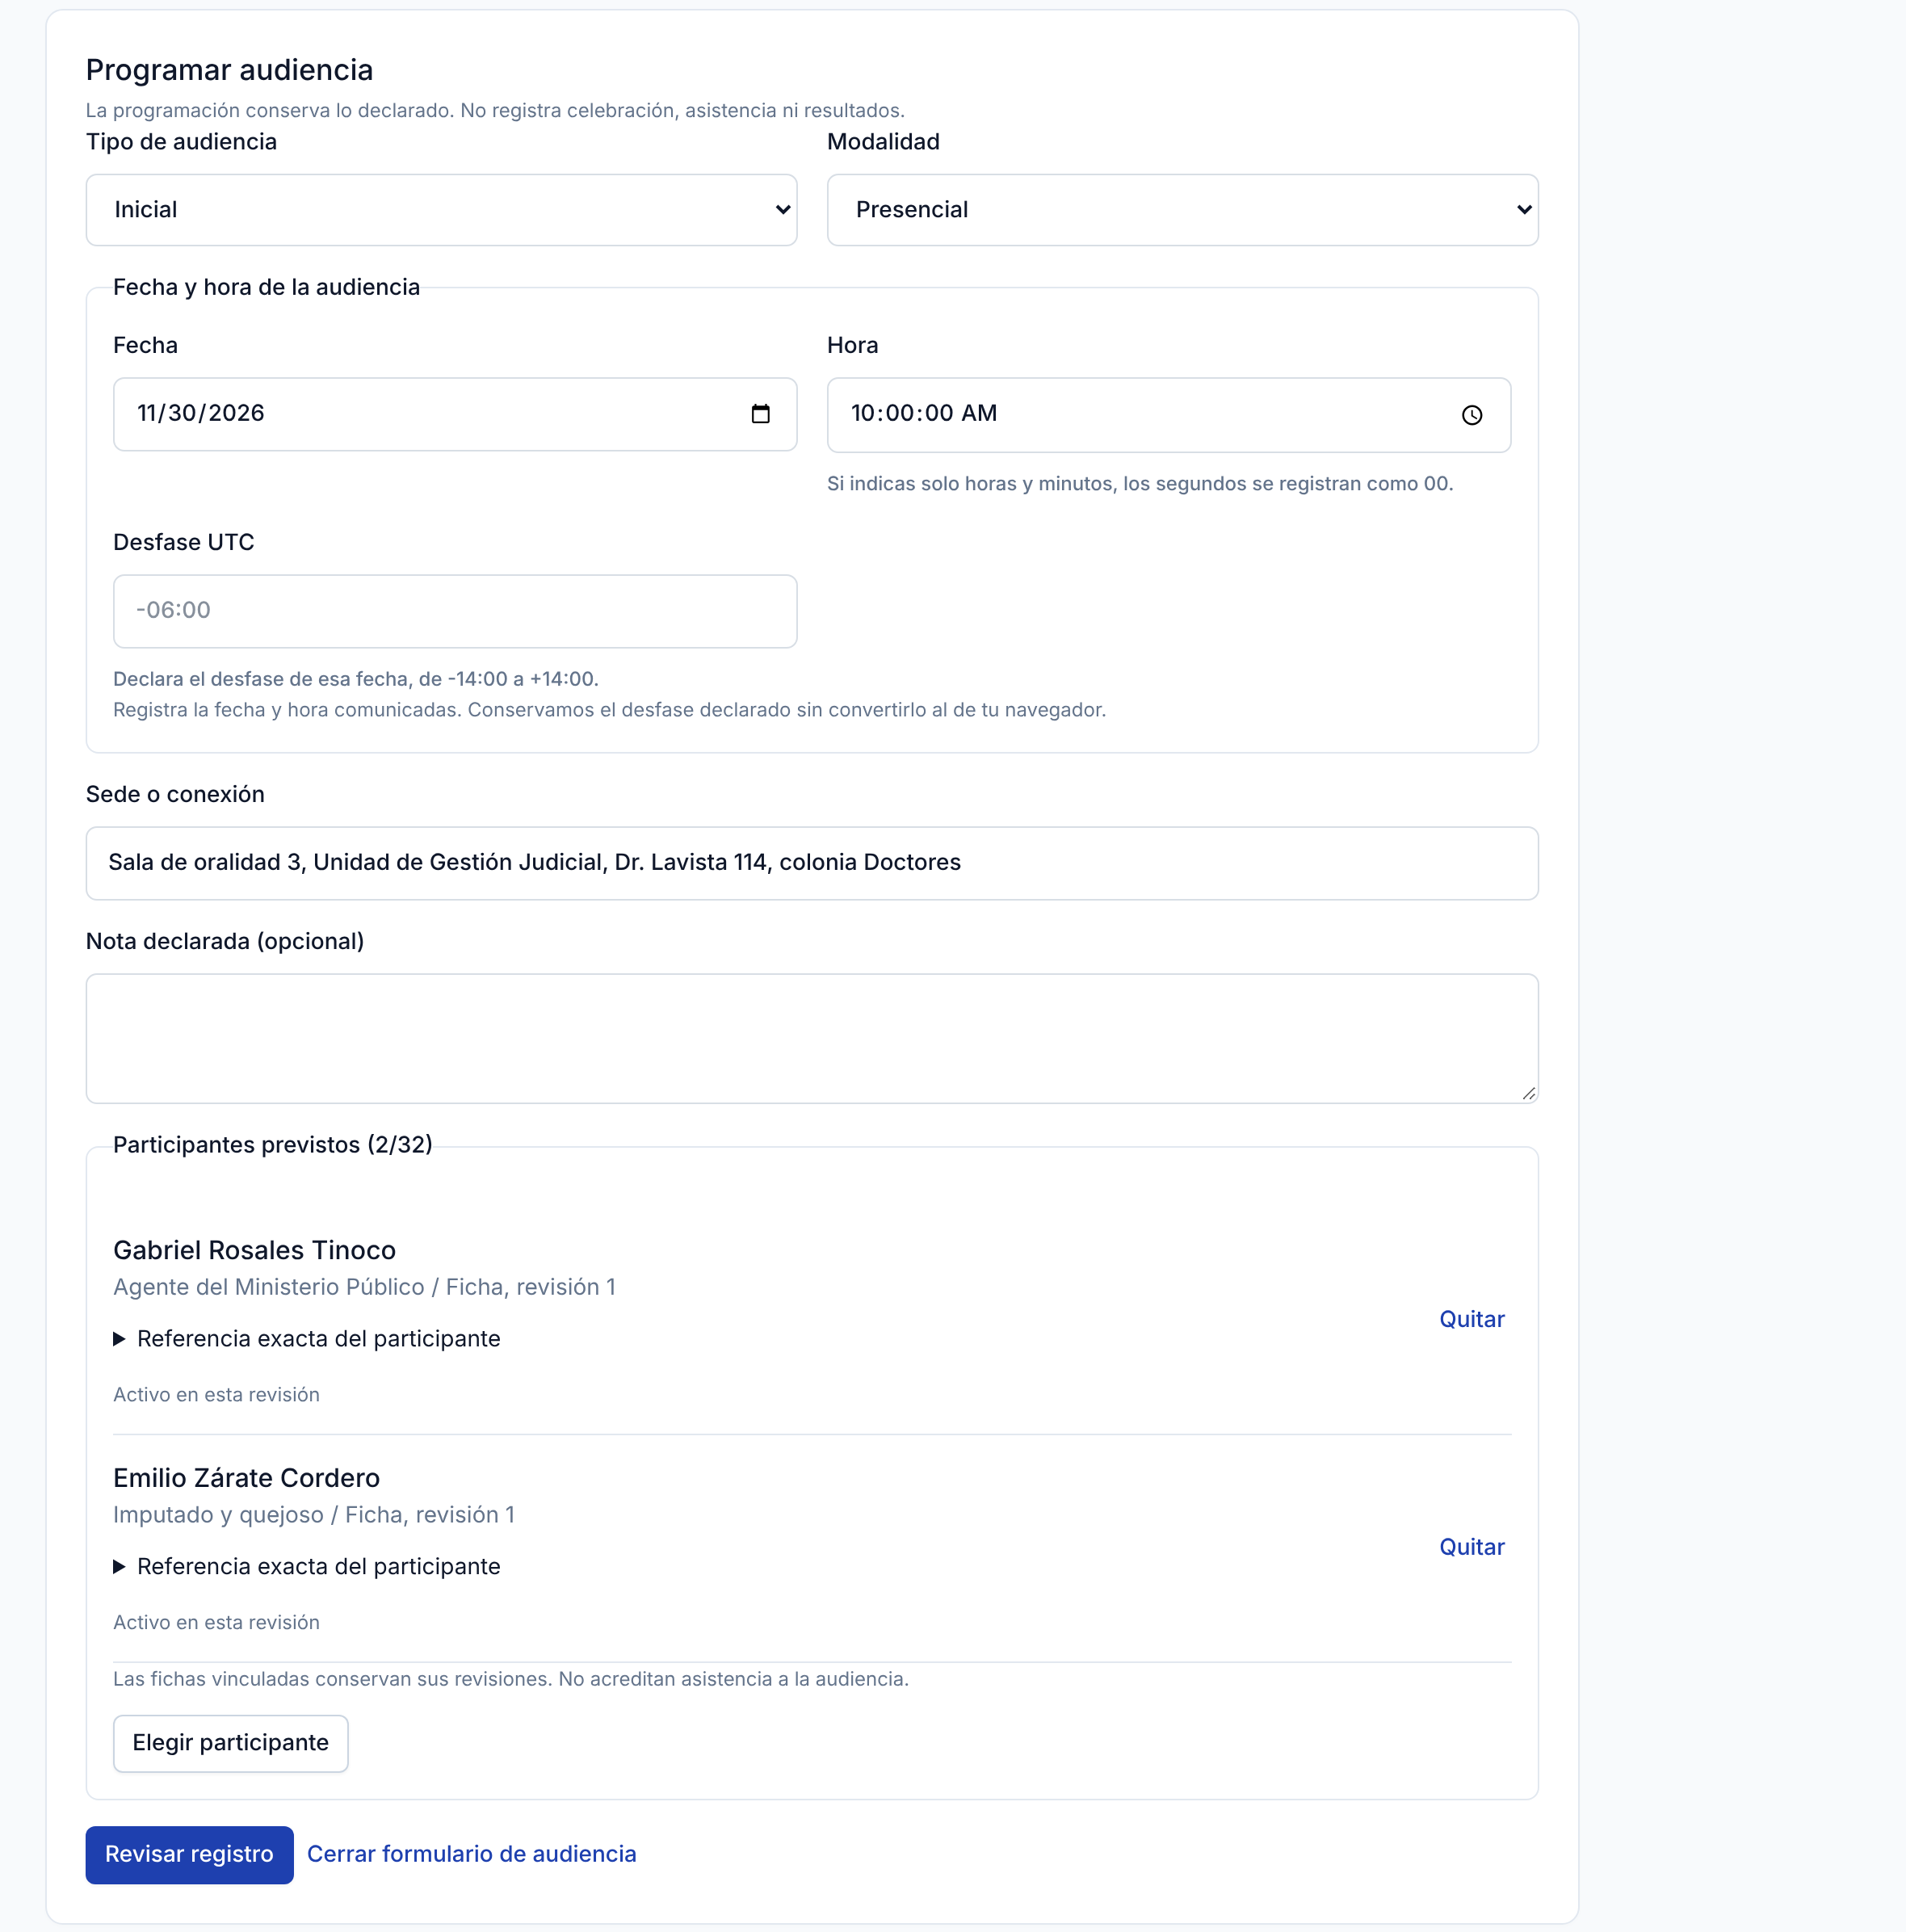
\includegraphics[width=0.9\textwidth,height=0.8\textheight,keepaspectratio]{capturas/A-29-programar-audiencia.png}
  \caption{Programación de una audiencia.}
  \label{fig:manual-programar-audiencia}
\end{figure}

\resultado La audiencia aparece como \textbf{Programada} en la lista y en la
\textbf{Agenda}.

\nota{Programar no acredita que la audiencia se celebró; regístrelo después
en \textbf{Ver sesiones y resultados}. Retirar un resultado conserva su
historia y no anula el acto informado.}

% ---------------------------------------------------------------------
\section{Medidas cautelares}\label{sec:medidas-cautelares}

\paraque Registra las decisiones sobre medidas cautelares (imposición,
modificación, revocación, sustitución) y lleva el registro de cada medida.

\disponible Administrador y Litigante (registran); Asistente legal
(consulta).

\begin{table}[H]
  \centering
  \caption{Acciones en Medidas cautelares.}\label{tab:acciones-medidas}
  \begin{tabularx}{\textwidth}{L{4.8cm} Y}
    \toprule
    \textbf{Botón} & \textbf{Qué hace} \\
    \midrule
    \textbf{Registrar decisión cautelar}   & Registra una decisión y sus efectos sobre las medidas. \\
    \textbf{Consultar decisión cautelar}   & Muestra la decisión con sus fuentes. \\
    \textbf{Consultar medida}              & Muestra el registro de una medida y su historia. \\
    \textbf{Rectificar registro}           & Corrige el registro de una medida, con su motivo. \\
    \textbf{Marcar registro por error}     & Señala un registro capturado por error. \\
    \bottomrule
  \end{tabularx}
\end{table}

\pasos\ Registrar una decisión cautelar:
\begin{enumerate}
  \item En la pestaña \textbf{Medidas cautelares}, haga clic en
        \textbf{Registrar decisión cautelar}.
  \item Indique la \textbf{Autoridad}, la \textbf{Precisión de decisión}
        y la fecha, la \textbf{Justificación} y el \textbf{Resultado}
        (\textbf{Cambios en medidas} o \textbf{Sin cambio en medidas}).
  \item Con \textbf{Cambios en medidas}, el formulario muestra el
        \textbf{Efecto 1}: elija la \textbf{Acción de medida}
        (\textbf{Imponer}, \textbf{Confirmar}, \textbf{Modificar},
        \textbf{Revocar}, \textbf{Cesar} o \textbf{Sustituir}), la persona
        (\textbf{Elegir sujeto}), la \textbf{Clase de medida}, las
        \textbf{Condiciones} y la vigencia. Para otro efecto, haga clic en
        \textbf{Agregar efecto}.
  \item Indique si la decisión viene de una audiencia (inicial o cautelar)
        o es independiente.
  \item Haga clic en \textbf{Revisar decisión} y después en
        \textbf{Confirmar decisión}.
\end{enumerate}

\begin{figure}[H]
  \centering
  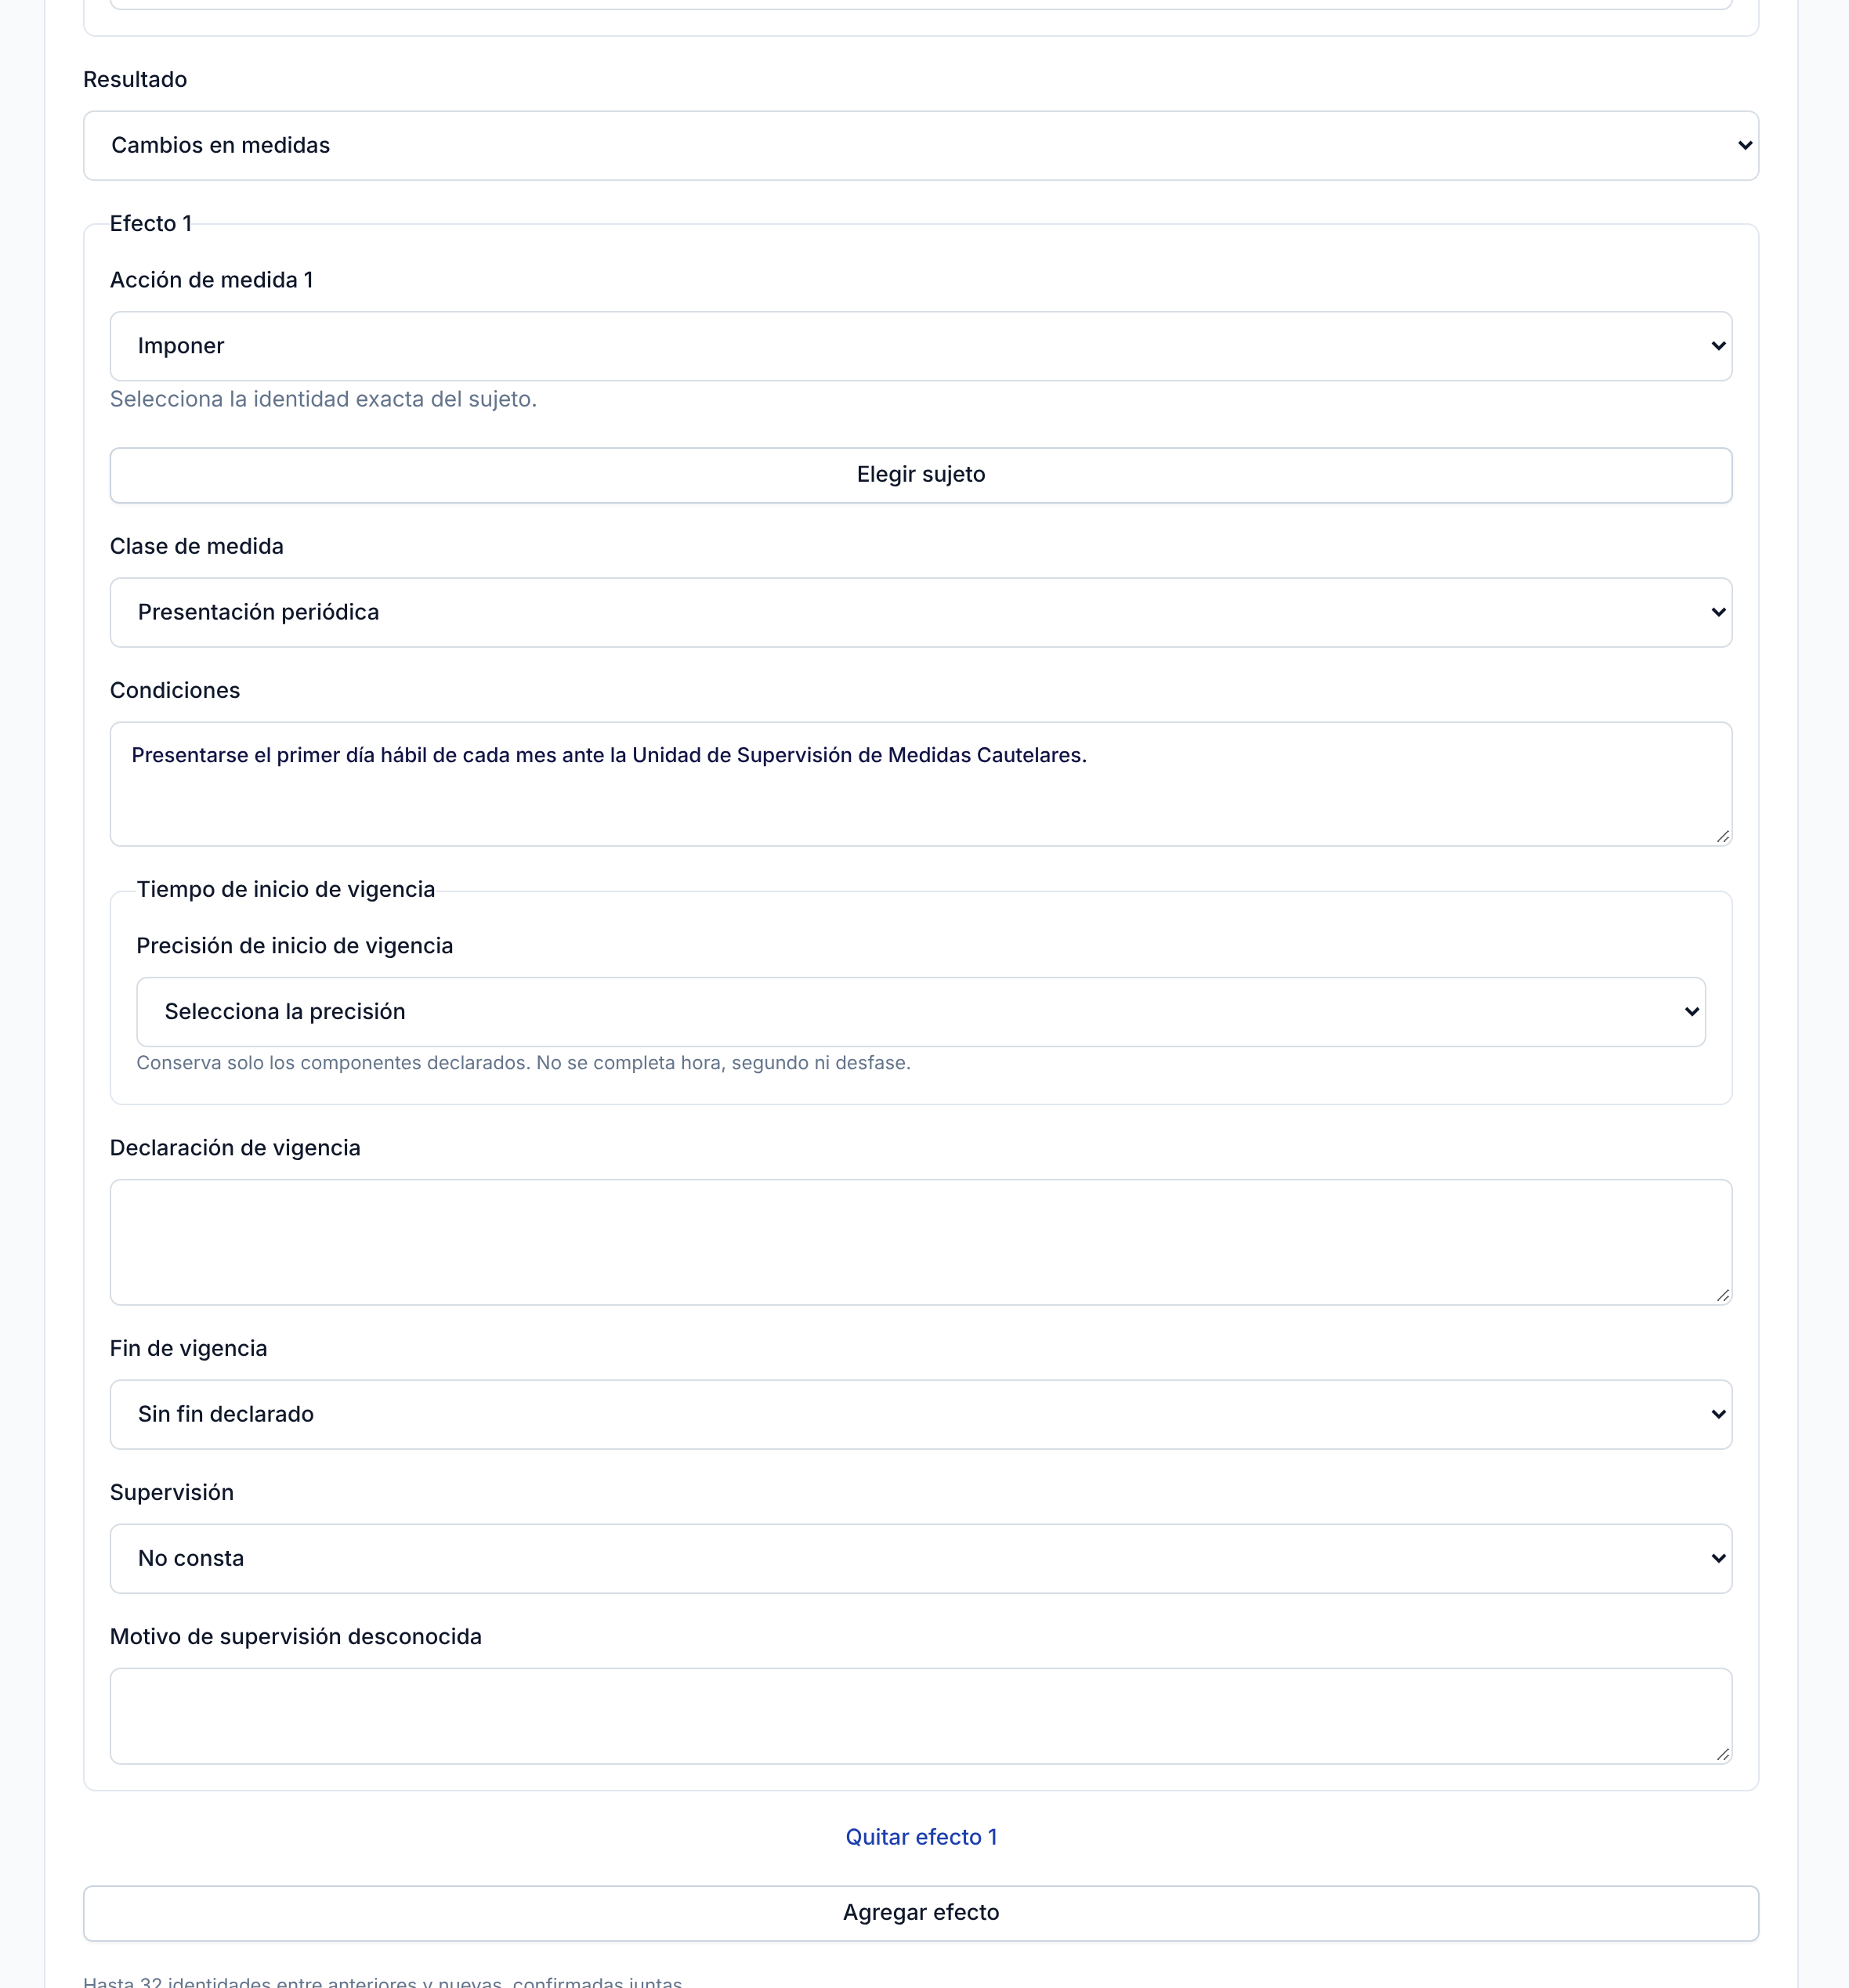
\includegraphics[width=0.9\textwidth,height=0.8\textheight,keepaspectratio]{capturas/A-30-decision-cautelar.png}
  \caption{Registro de una decisión cautelar.}
  \label{fig:manual-decision-cautelar}
\end{figure}

\resultado La decisión y las medidas afectadas aparecen en la pestaña.

\nota{Las audiencias cautelares se programan desde la pestaña
\textbf{Audiencias} (\cref{sec:audiencias}). El estado del expediente no
determina la vigencia jurídica de una medida.}

% ---------------------------------------------------------------------
\section{Resoluciones y notificaciones}\label{sec:resoluciones}

\paraque Registra las resoluciones del expediente y, dentro de cada una,
sus notificaciones.

\disponible Administrador y Litigante (registran); Asistente legal
(consulta).

\begin{table}[H]
  \centering
  \caption{Acciones en Resoluciones.}\label{tab:acciones-resoluciones}
  \begin{tabularx}{\textwidth}{L{4.8cm} Y}
    \toprule
    \textbf{Botón} & \textbf{Qué hace} \\
    \midrule
    \textbf{Registrar resolución}          & Registra un auto, una sentencia u otra resolución. \\
    \textbf{Corregir resolución} / \textbf{Retirar resolución}
                                           & Corrige o retira el registro; retirar no anula el acto. \\
    \textbf{Ver notificaciones}            & Abre las notificaciones de esa resolución. \\
    \textbf{Registrar notificación}        & Registra cómo y a quién se notificó. \\
    \textbf{Ver historial de resolución}   & Muestra todas las versiones del registro. \\
    \bottomrule
  \end{tabularx}
\end{table}

\pasos\ Registrar una resolución y su notificación:
\begin{enumerate}
  \item En la pestaña \textbf{Resoluciones}, haga clic en
        \textbf{Registrar resolución}.
  \item Elija la \textbf{Clase de resolución} (\textbf{Auto u orden},
        \textbf{Sentencia} u \textbf{Otra clase}), el \textbf{Emisor}, la
        fecha de emisión y el resumen.
  \item Haga clic en \textbf{Preparar registro} y después en
        \textbf{Confirmar registro}.
  \item En la resolución registrada, haga clic en \textbf{Ver notificaciones}
        y luego en \textbf{Registrar notificación}.
  \item Elija el \textbf{Carácter de notificación}, el
        \textbf{Medio de notificación}, el \textbf{Contexto de notificación}
        y el \textbf{Resultado declarado}. Confirme igual que en el paso 3.
\end{enumerate}

\begin{figure}[H]
  \centering
  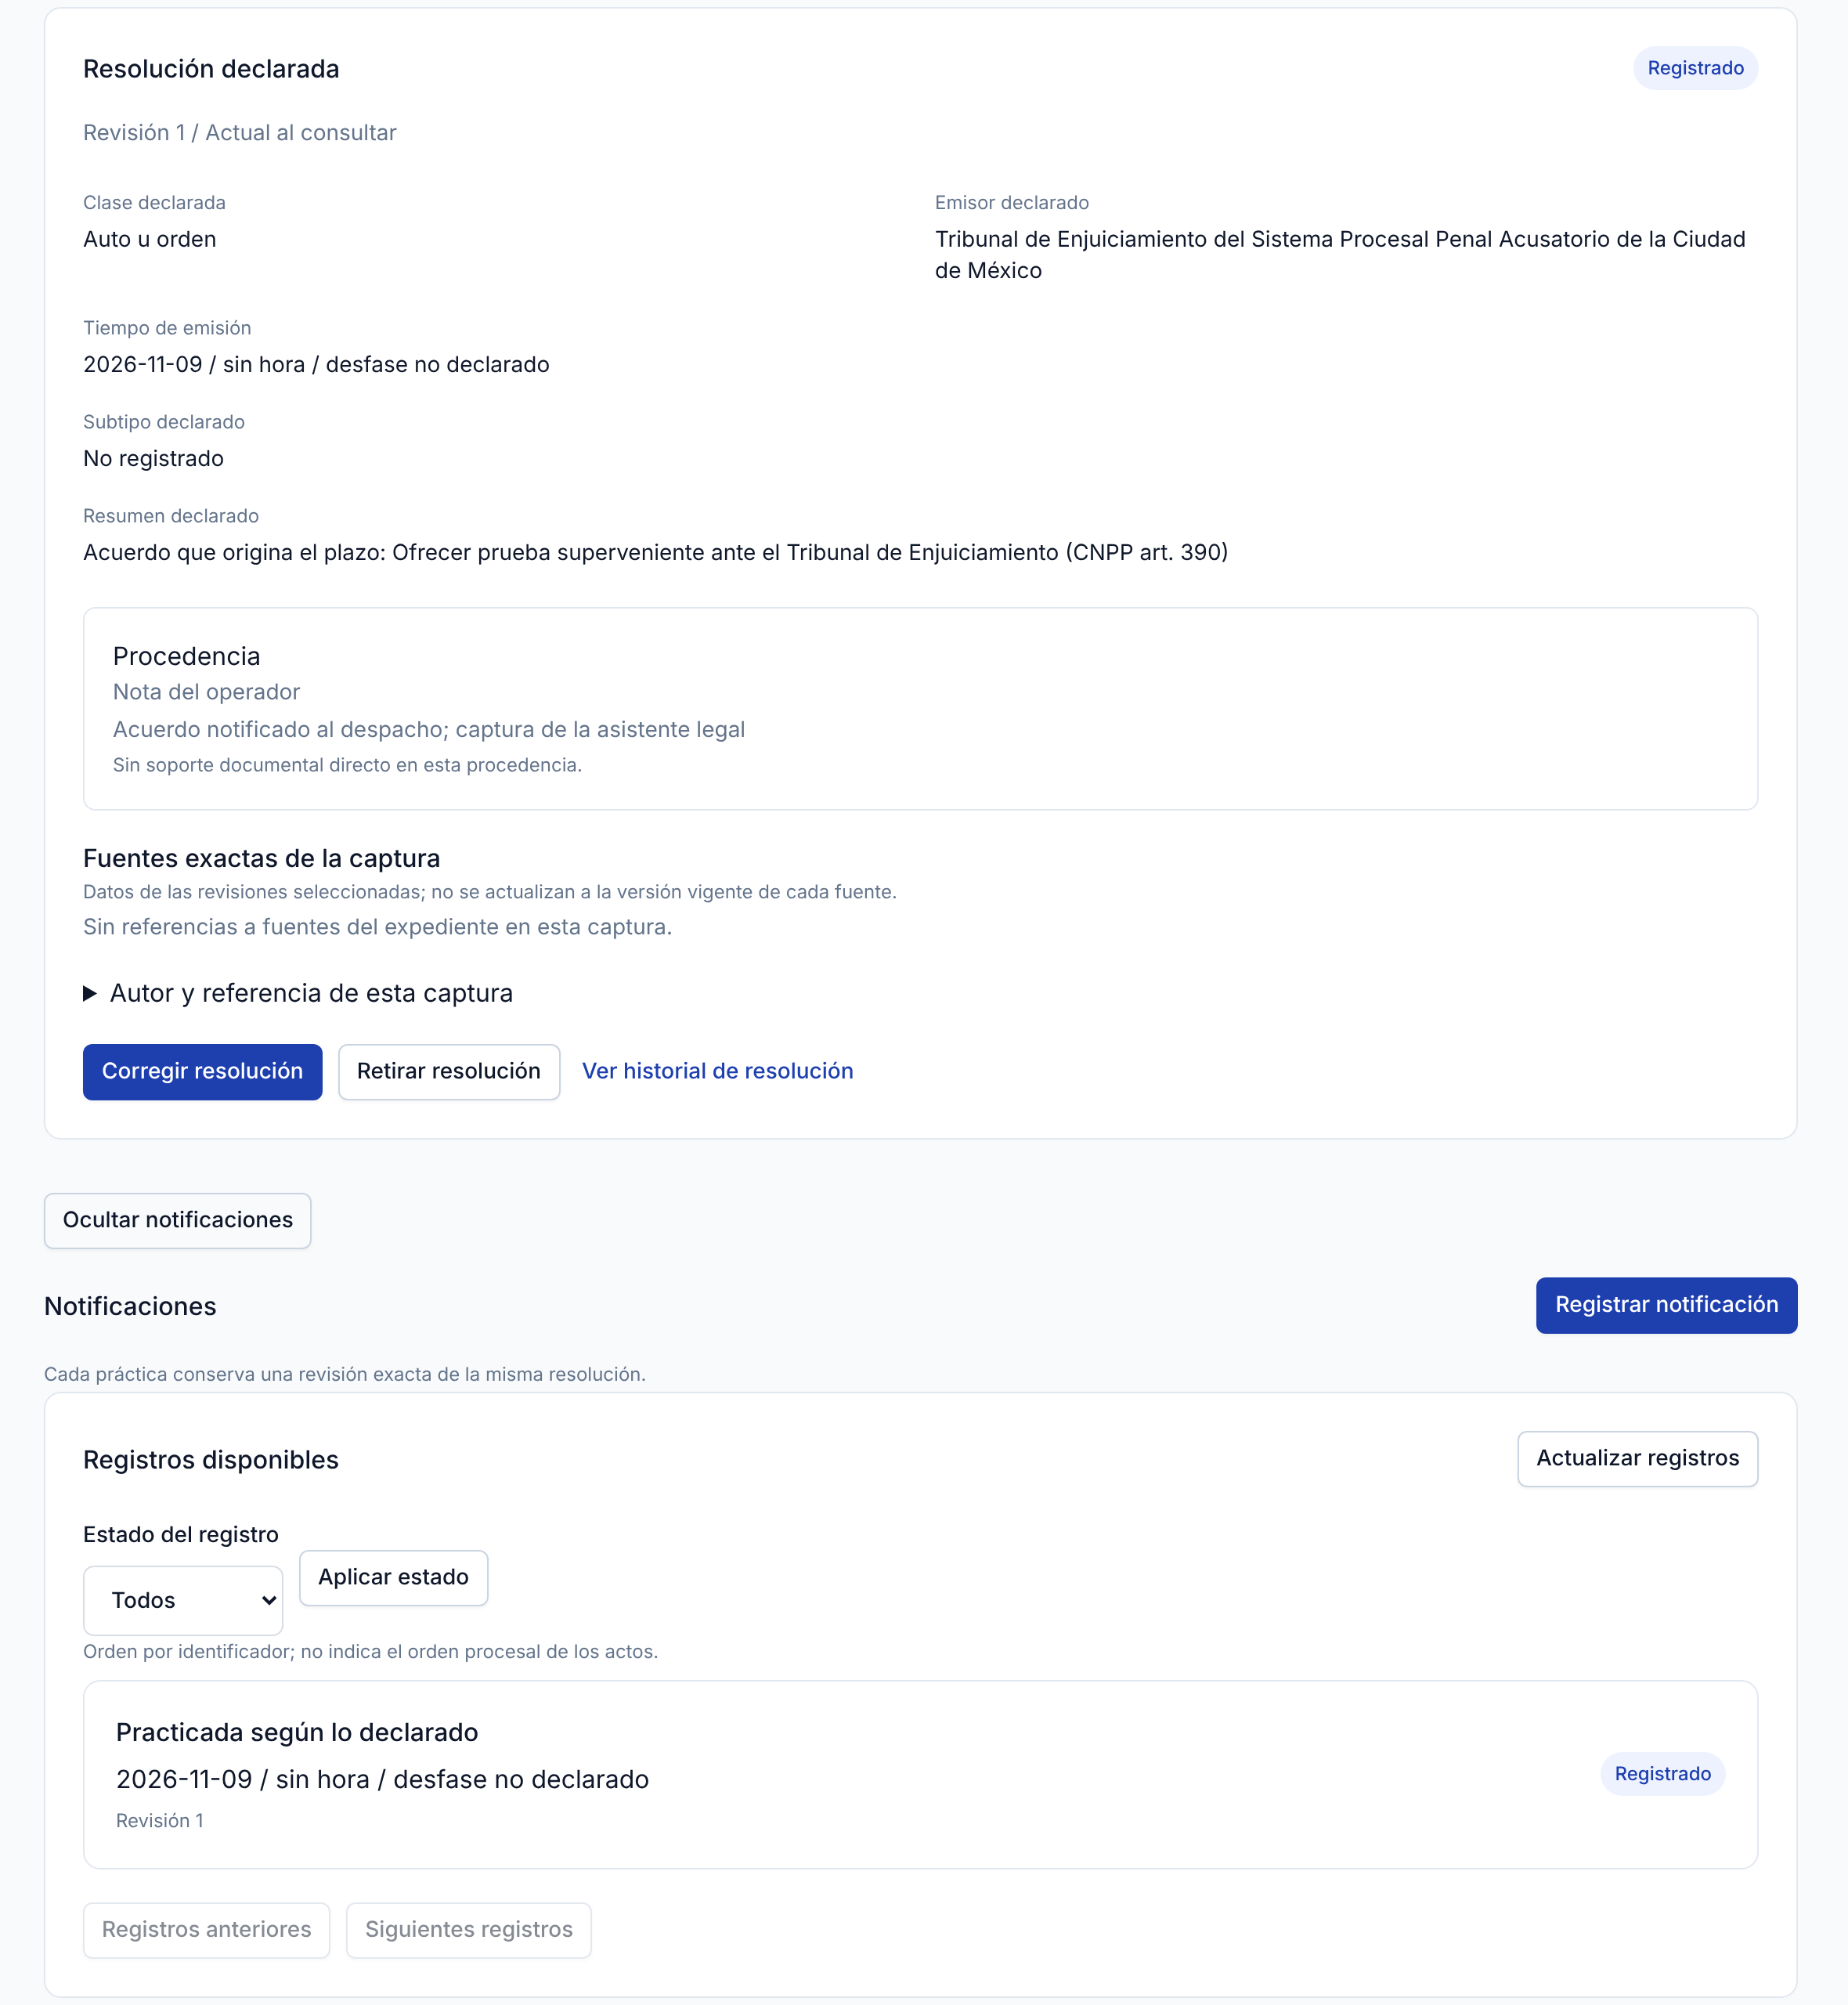
\includegraphics[width=0.9\textwidth,height=0.8\textheight,keepaspectratio]{capturas/A-31-resoluciones.png}
  \caption{Resoluciones y notificaciones.}
  \label{fig:manual-resoluciones}
\end{figure}

\resultado Qadra muestra \textbf{Registro guardado.} y la resolución aparece
en \textbf{Registros disponibles} con su notificación.

% ---------------------------------------------------------------------
\section{Recursos}\label{sec:recursos}

\paraque Registra recursos de revocación y apelación, sus actos y su
relación con audiencias y plazos.

\disponible Administrador y Litigante (registran); Asistente legal
(consulta).

\begin{table}[H]
  \centering
  \caption{Acciones en Recursos.}\label{tab:acciones-recursos}
  \begin{tabularx}{\textwidth}{L{4.8cm} Y}
    \toprule
    \textbf{Botón} & \textbf{Qué hace} \\
    \midrule
    \textbf{Registrar recurso}             & Registra una revocación o una apelación. \\
    \textbf{Registrar acto}                & Agrega interposición, admisión, inadmisibilidad, desistimiento o resolución. \\
    \textbf{Corregir recurso}              & Corrige los datos del recurso. \\
    \textbf{Archivar recurso} / \textbf{Reactivar recurso}
                                           & Ordena la lista; no declara desistimiento. \\
    \textbf{Vincular actividad}            & Relaciona una audiencia o un plazo existente. \\
    \textbf{Crear plazo}                   & Crea un plazo ya vinculado al recurso. \\
    \textbf{Crear audiencia de recurso}    & Programa una audiencia ya vinculada al recurso. \\
    \bottomrule
  \end{tabularx}
\end{table}

\pasos\ Registrar un recurso:
\begin{enumerate}
  \item En la pestaña \textbf{Recursos}, haga clic en
        \textbf{Registrar recurso}.
  \item Elija el \textbf{Tipo de recurso} (\textbf{Revocación} o
        \textbf{Apelación}) y llene los datos: parte impugnada, personas
        recurrentes, motivos, \textbf{Modalidad del recurso}, autoridades y
        \textbf{Referencia de la resolución}.
  \item Haga clic en \textbf{Preparar registro} y después en
        \textbf{Confirmar registro}.
\end{enumerate}

\begin{figure}[H]
  \centering
  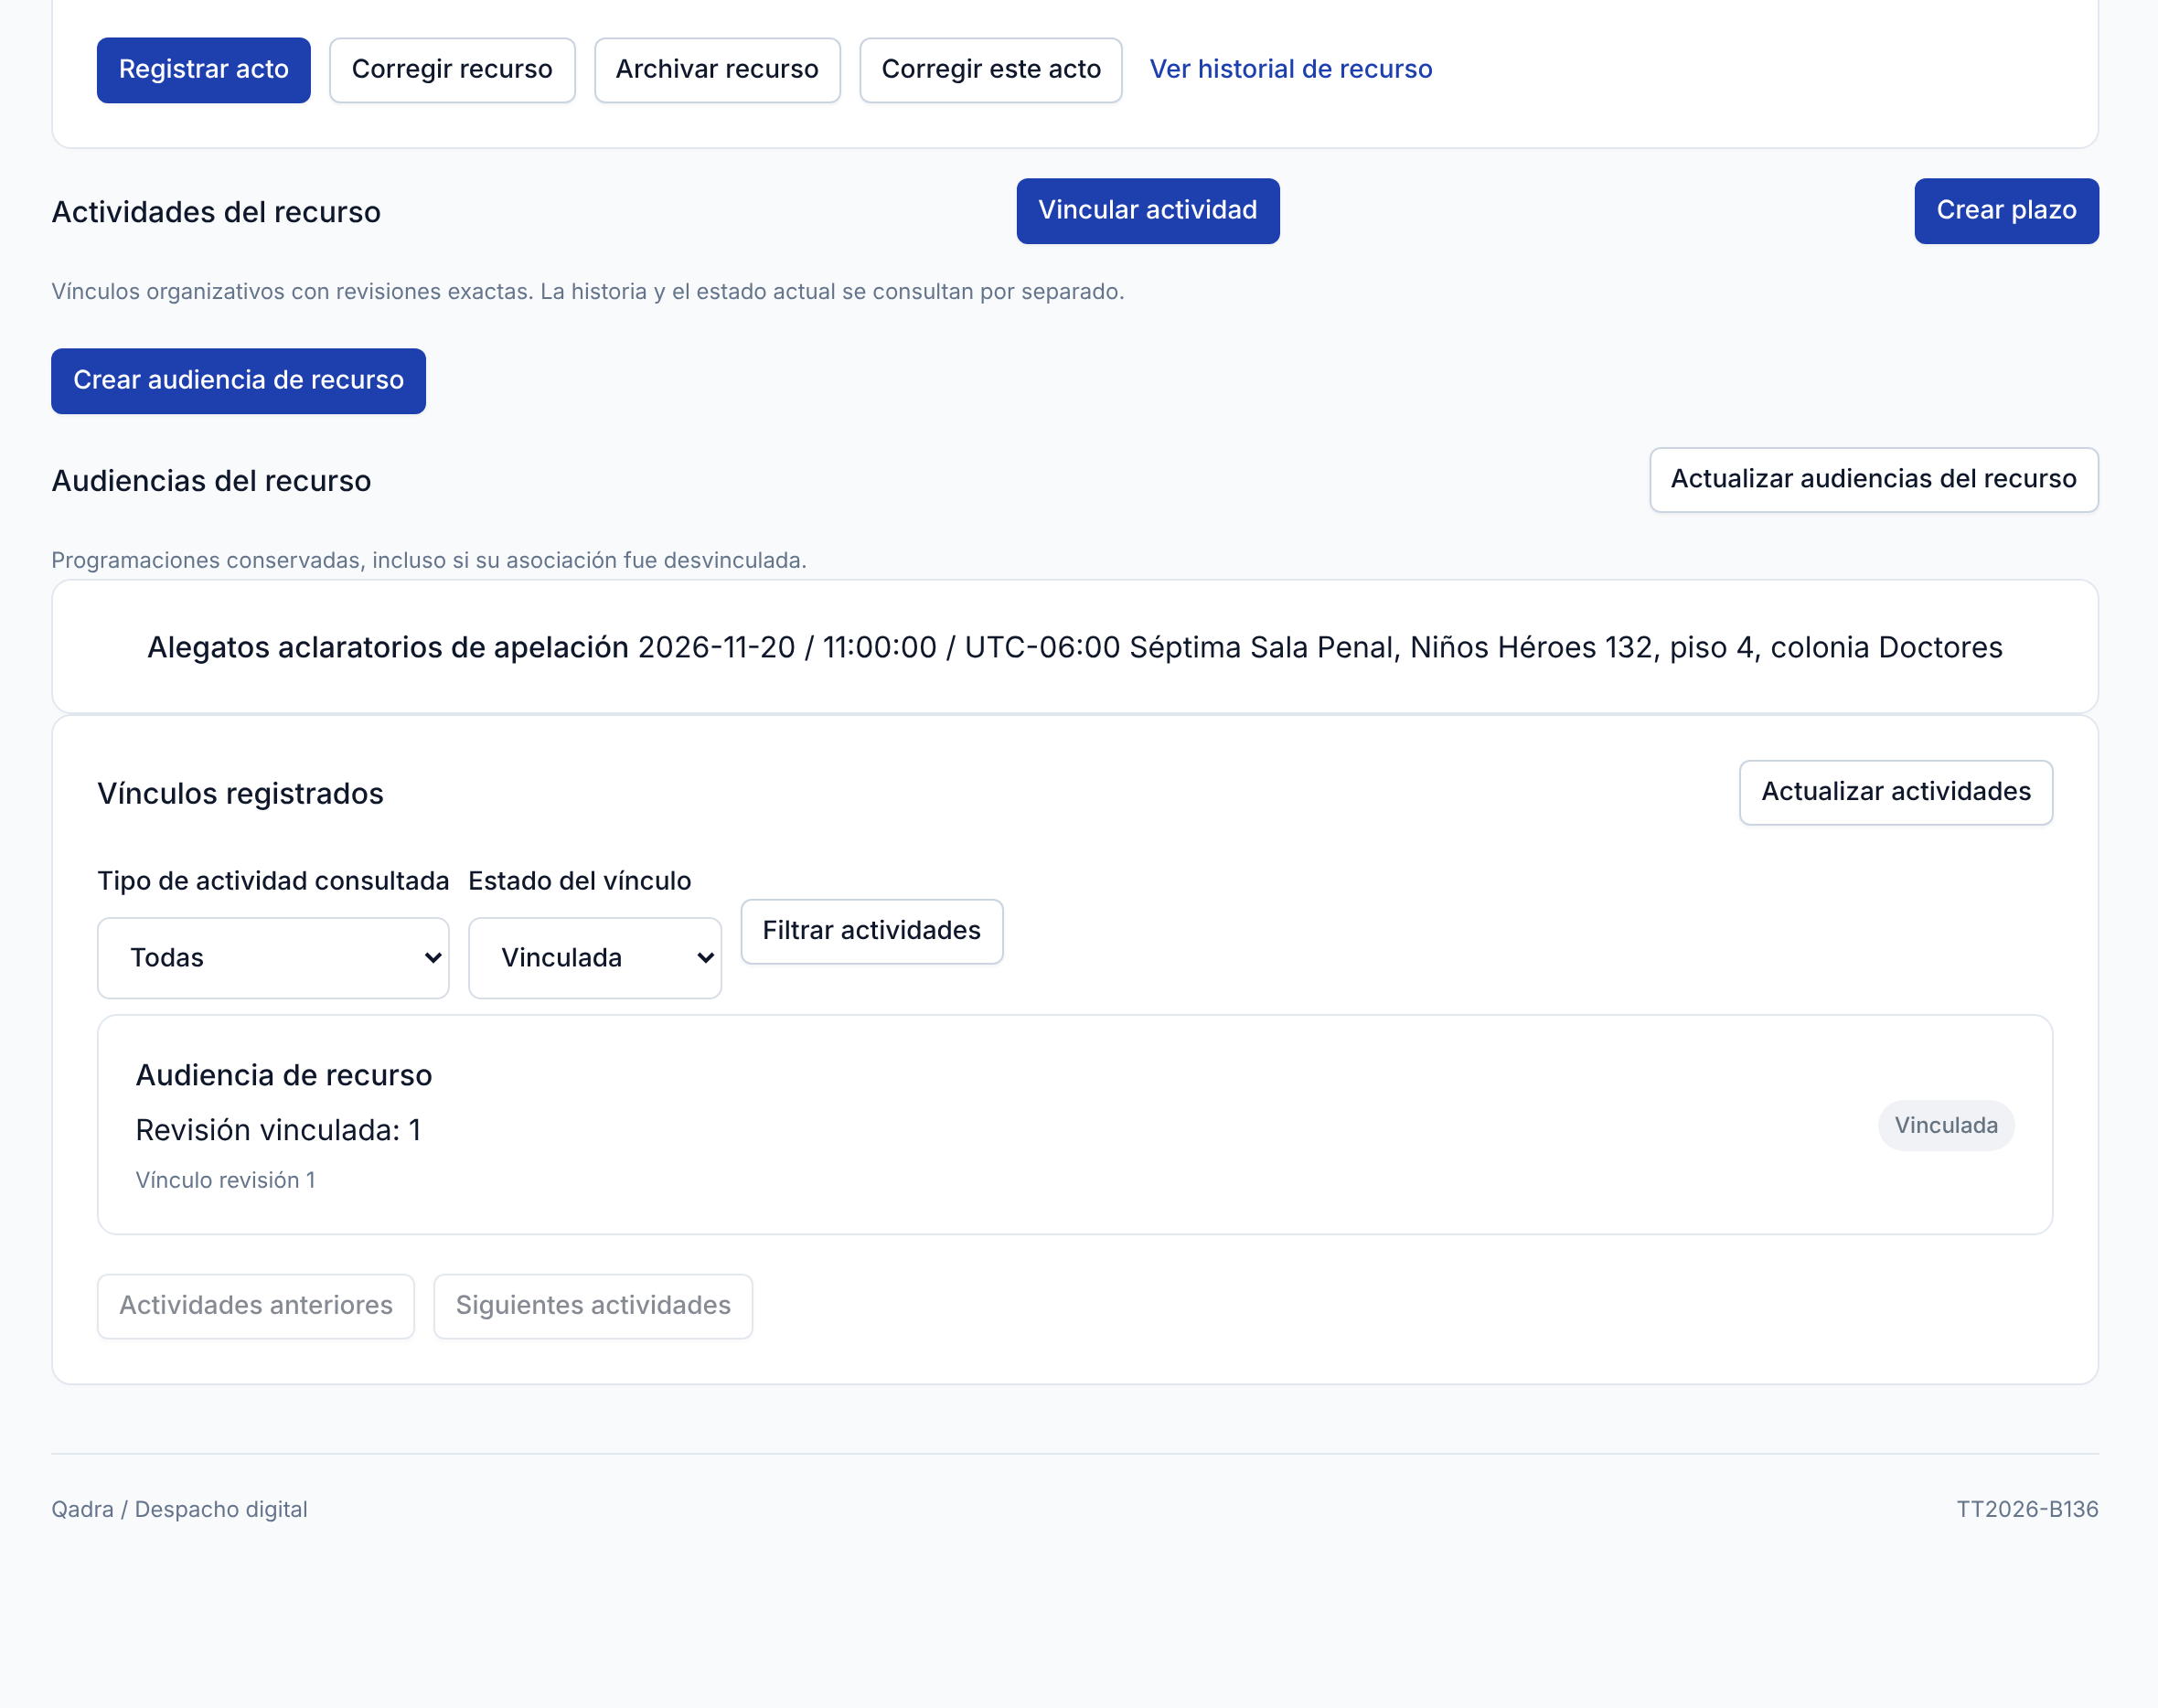
\includegraphics[width=0.9\textwidth,height=0.8\textheight,keepaspectratio]{capturas/A-32-recursos.png}
  \caption{Recursos procesales.}
  \label{fig:manual-recursos}
\end{figure}

\resultado El recurso aparece en \textbf{Recursos del expediente}. Desde ahí
puede registrar sus actos y vincular actividades.

% ---------------------------------------------------------------------
\section{Plazos}\label{sec:plazos}

\paraque Calcula el vencimiento de un plazo a partir de su fuente, su regla
y el calendario judicial, y registra si ya se atendió.

\disponible Administrador y Litigante (registran); Asistente legal
(consulta).

\begin{table}[H]
  \centering
  \caption{Acciones en Plazos.}\label{tab:acciones-plazos}
  \begin{tabularx}{\textwidth}{L{4.4cm} Y}
    \toprule
    \textbf{Botón} & \textbf{Qué hace} \\
    \midrule
    \textbf{Registrar plazo}          & Crea un plazo y calcula su vencimiento. \\
    \textbf{Corregir plazo}           & Corrige fuente, regla, calendario o responsable. \\
    \textbf{Revisar seguimiento}      & Aparece cuando un cambio en la fuente o la regla requiere su revisión. \\
    \textbf{Declarar atención}        & Registra que el plazo ya se atendió. \\
    \textbf{Retirar plazo}            & Retira el plazo; su cálculo queda en el historial. \\
    \textbf{Ver historial de plazo}   & Muestra cada cálculo y quién lo hizo. \\
    \bottomrule
  \end{tabularx}
\end{table}

\pasos\ Registrar un plazo:
\begin{enumerate}
  \item En la pestaña \textbf{Plazos}, haga clic en \textbf{Registrar plazo}.
  \item Escriba el \textbf{Título del plazo}.
  \item En \textbf{Regla aplicable}, haga clic en
        \textbf{Elegir perfil exacto}, elija el perfil, abra su revisión con
        \textbf{Consultar perfil revisión} y confirme con
        \textbf{Usar este perfil exacto}. En \textbf{Cuando cambie el
        perfil} elija \textbf{Conservar esta revisión} o
        \textbf{Seguir cambios y solicitar revisión}.
  \item En \textbf{Responsable}, haga clic en
        \textbf{Elegir responsable} y elija a la persona que lo atenderá.
  \item En \textbf{Fuente exacta del inicio}, elija el
        \textbf{Tipo de fuente} (\textbf{Resolución},
        \textbf{Notificación} o \textbf{Resultado de audiencia}), haga clic
        en \textbf{Elegir fuente exacta}, abra la revisión con
        \textbf{Consultar revisiones de la fuente} y vincúlela con
        \textbf{Vincular esta revisión}. Elija también cómo seguir los
        cambios de la fuente.
  \item En \textbf{Calendario}, haga clic en
        \textbf{Elegir calendario exacto} y elija su revisión con
        \textbf{Usar este calendario exacto}; para seguir sus cambios,
        elija \textbf{Seguir cambios del calendario}.
  \item Complete la \textbf{Declaración de aplicabilidad}, el
        \textbf{Localizador de aplicabilidad}, las preguntas sobre el
        ámbito del perfil, la incidencia sin resolver y cada condición del
        perfil.
  \item Haga clic en \textbf{Preparar plazo}. Revise el resultado en
        \textbf{Cálculo conservado en esta revisión} y los pasos en
        \textbf{Ver pasos del cómputo}.
  \item Marque \textbf{Revisé las declaraciones, fuentes, políticas y el
        resultado a guardar} y haga clic en \textbf{Confirmar plazo}. Si
        necesita cambiar algo, use \textbf{Volver al borrador}.
\end{enumerate}

\begin{figure}[H]
  \centering
  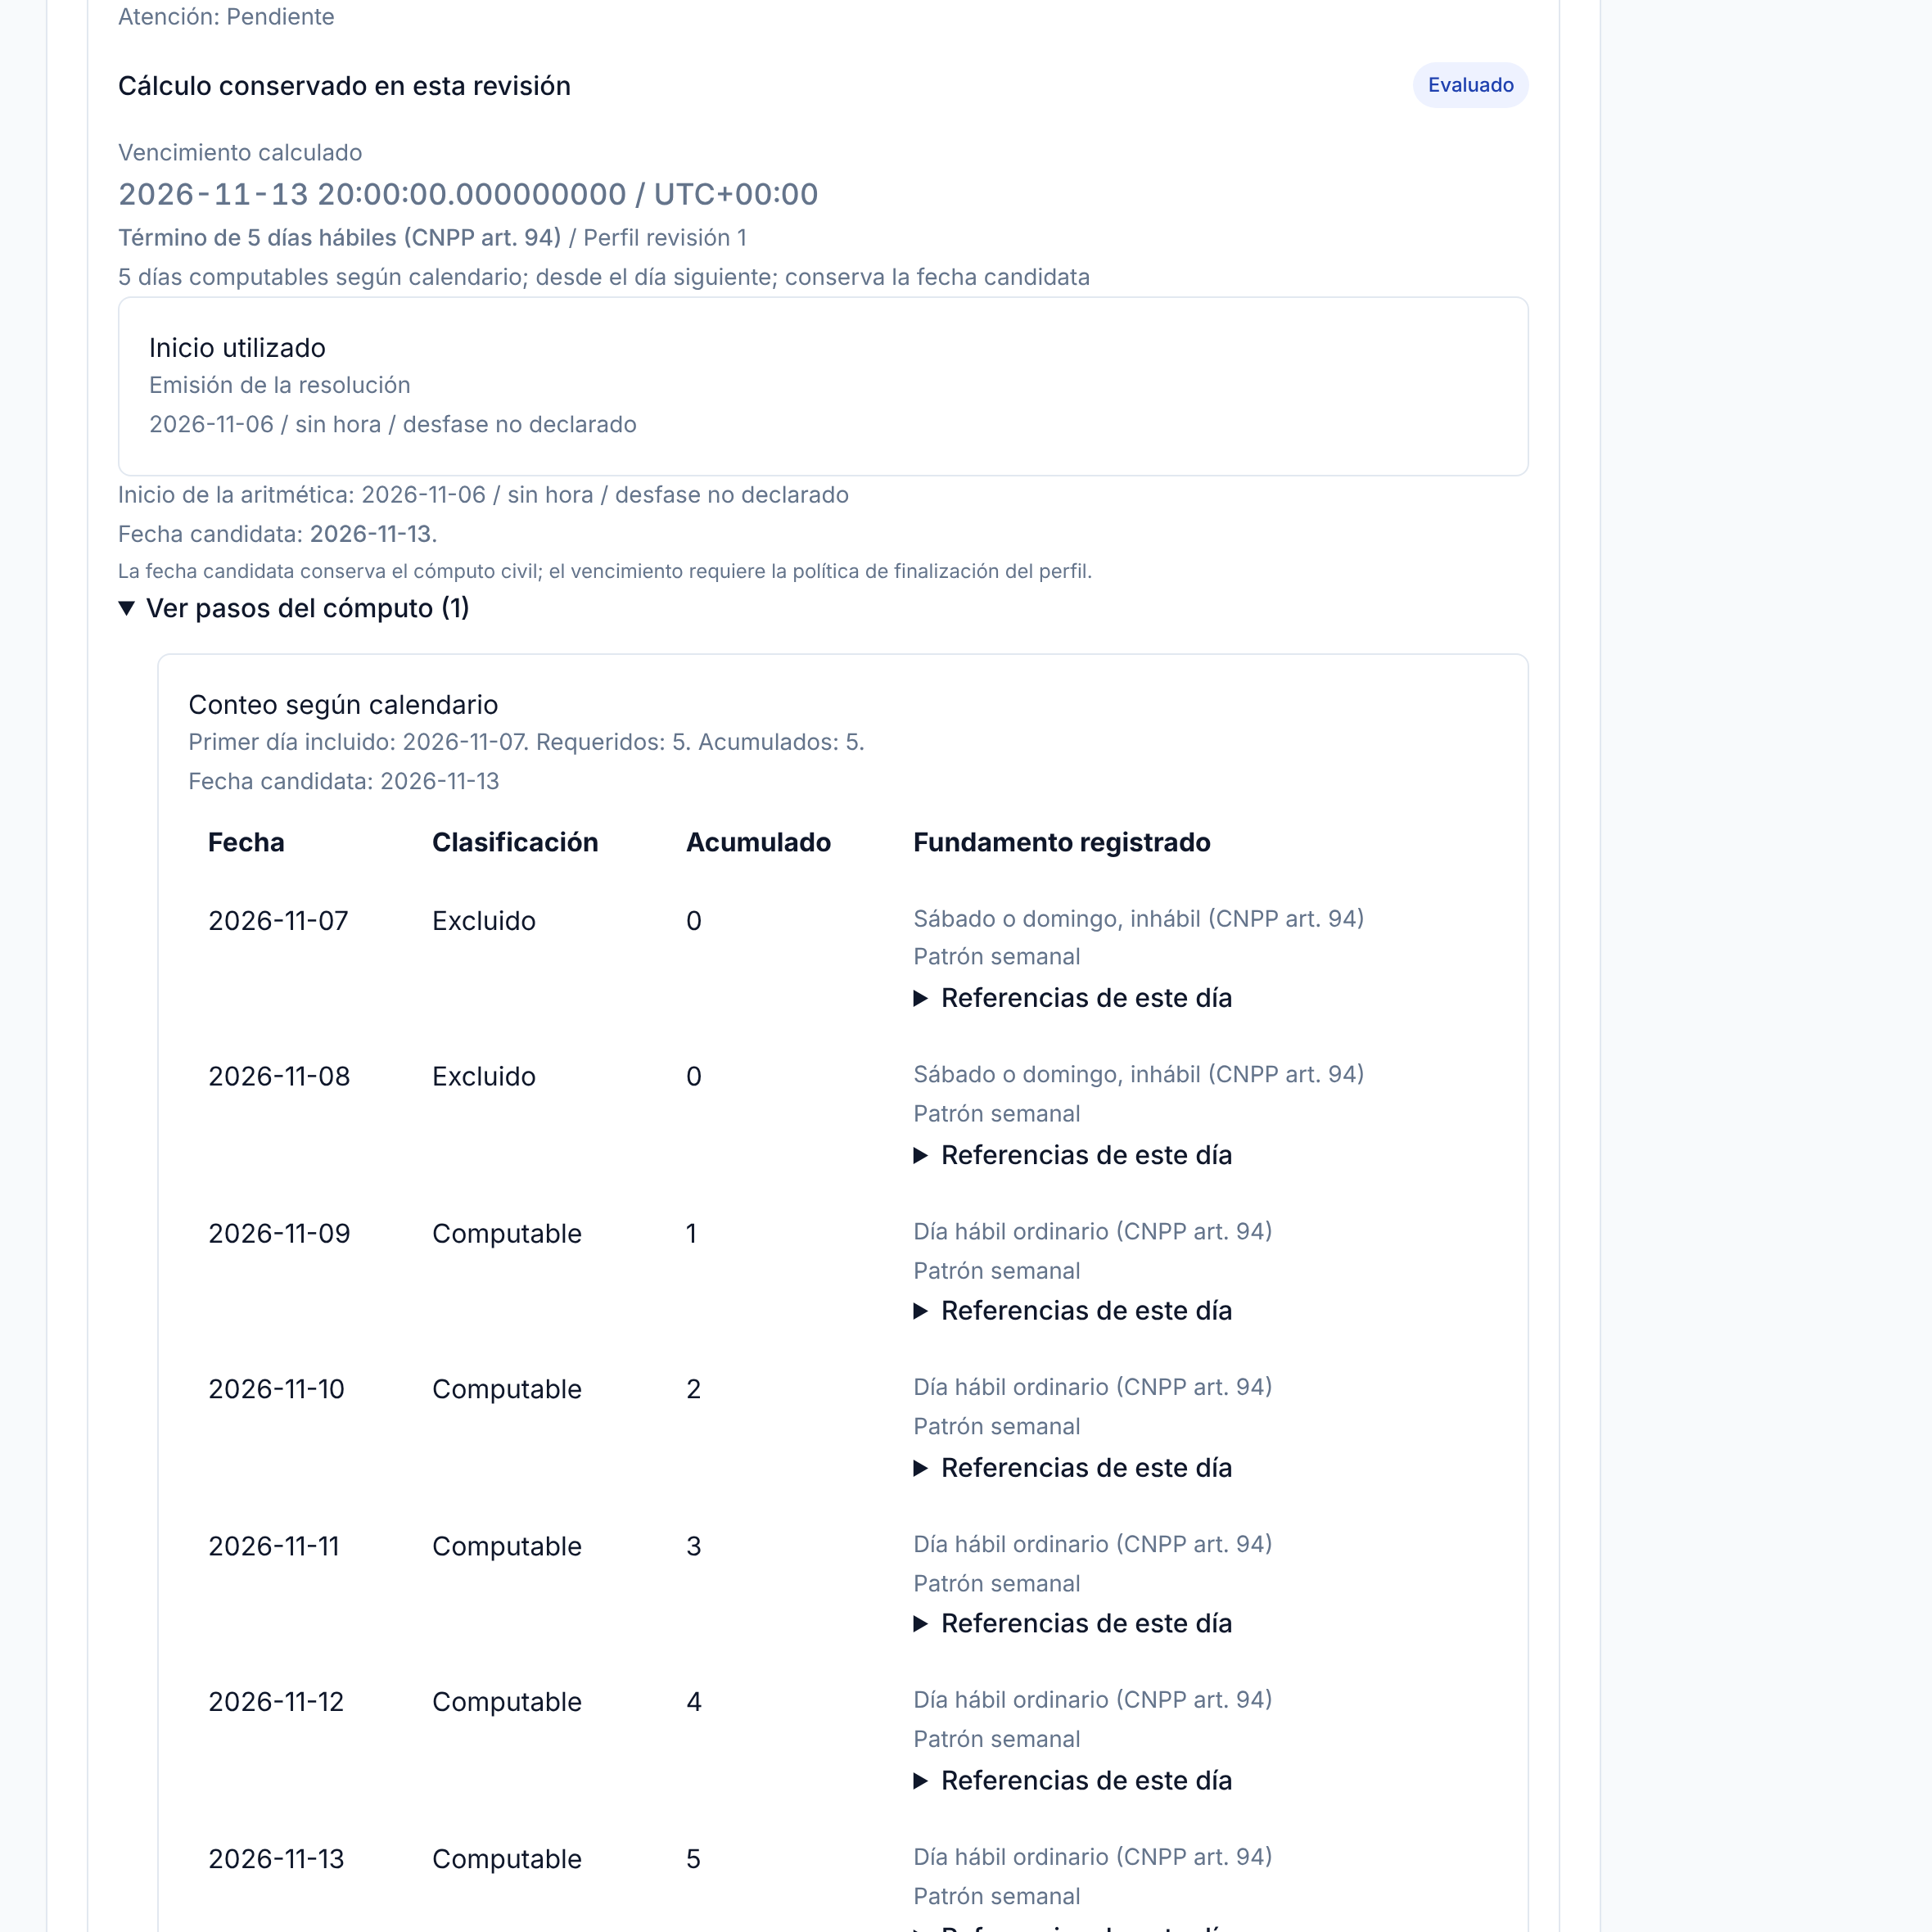
\includegraphics[width=0.9\textwidth,height=0.8\textheight,keepaspectratio]{capturas/A-33-registrar-plazo.png}
  \caption{Registro de un plazo.}
  \label{fig:manual-registrar-plazo}
\end{figure}

\resultado El plazo aparece en \textbf{Seguimiento de plazos} con su
\textbf{Vencimiento para seguimiento} y en la \textbf{Agenda}.

\begin{itemize}
  \item Si falta información, el plazo queda con \textbf{Cálculo bloqueado}:
        Qadra no inventa un vencimiento. Complete lo que falta con
        \textbf{Corregir plazo}.
  \item Elegir un responsable no le da acceso al expediente.
  \item Declarar atención o leer una alerta no acredita por sí solo una
        presentación válida.
\end{itemize}
